\documentclass[12pt]{article}
\setlength{\oddsidemargin}{0.in}
\setlength{\textwidth}{6.5in}
\setlength{\topmargin}{-0.25in}
\setlength{\textheight}{8.25in}

% Skip space between paragraphs
\setlength{\parskip}{.1in}

% Do not put numbers in section headings
\setcounter{secnumdepth}{0}

% Indent paragraphs 0. in
\setlength{\parindent}{0.in}

% Use the natbib package for the bibliography
\usepackage[round]{natbib}
\bibliographystyle{sysbio}

% Use the graphicx package to incorporate and scale
% encapsulated postscript figures
\usepackage{graphicx}

% Make document single-spaced
\renewcommand{\baselinestretch}{1.0}

%\newcommand{\ncat}{\mbox{$n_{\mbox{\tiny cat}}$}}
\newcommand{\ncat}{n_c}

\begin{document}

\section{The FLEXCAT model for among-site rate heterogeneity}
\subsubsection{Paul O. Lewis (6 May 2006)}

This document represents my notes on a new Bayesian model (the FLEXCAT model) for among-site rate heterogeneity that has the following features. This document is not intended to be a manuscript because it is much too detailed and does not provide an appropriate introduction or discussion to the topic, but I have worked out here all details of the FLEXCAT model and thus writing a paper from these notes should be straightforward.

\begin{itemize}
\item The number of rate categories is flexible, and is not fixed. A reversible jump MCMC approach allows the model to jump among different numbers of rate categories to find the number that is appropriate. This has several advantages. First, a dataset that can be described adequately with 2 rate categories will run much faster than a typical G+I model, which normally involves 5 rate categories (1 invariant category plus 4 gamma categories). Second, this approach allows the researcher to discover the number of rate categories that is appropriate, rather than having to specify a number.
\item The probabilities of each rate category are estimated rather than being assumed equal to the inverse of the number of categories. There are two advantages to this approach. First, the researcher can learn more about the distribution of rates if the probability of each rate category is estimated. Second, the model is better behaved in terms of posterior predictive variance. Consider a discrete gamma rate model with four categories in a situation involving considerable rate heterogeneity. The discrete gamma model in such cases will specify a large relative rate for the last category, and this category is responsible for generating fully one fourth of the sites in posterior predictive simulations, even though far fewer than one fourth of the sites in the observed data matrix were evolving at this high rate. As a result, the posterior predictive loss approach detects much gratuitous variability in the posterior predictive distribution and penalizes the discrete gamma model heavily, often making a discrete gamma model score worse than a model that assumes no rate heterogeneity.
\item Finally, the relative rates used to represent each category in the FLEXCAT model are also estimated, and thus are not assumed to be gamma distributed. The assumption of a gamma distribution for relative rates has always been for convenience rather than biological realism, and in doing away with this assumption the FLEXCAT model provides a much more realistic picture of the among site rate heterogeneity present in a data set.
\end{itemize}

The likelihood component of the FLEXCAT model is identical to the Unit Mean General Discrete Distribution (UGDD) model descibed by \citet{KosakovskypondMuse2005}; however, the prior model and proposals needed for Bayesian reversible-jump MCMC analyses are unique to the FLEXCAT model.

In the discrete gamma model, the inverse of the shape parameter conveniently summarizes the amount of rate heterogeneity. The amount of rate heterogeneity can be summarized conveniently by a single value for the FLEXCAT model as well: the variance in relative rates can be estimated as follows:

\begin{eqnarray*}
\mbox{Var}(r) & = & \sum_{k=1}^{\ncat} r_k^2 \; p(k)
\end{eqnarray*}

\noindent where $\ncat$ is the number of rate categories, $r_k$ is the representative relative rate for category $k$ and $p(k)$ is the probability that category $k$ applies to any given site. In the (usual) case where $\ncat$ is itself a parameter, one could present instead the expected value of Var($r$), where the expectation is taken over all values of $\ncat$ and is estimated using MCMC.

The FLEXCAT model has a greater number of parameters than both the discrete gamma and invariant sites models. For example, if the number of rate categories is currently 4, the FLEXCAT model has 7 free parameters (1 parameter for the number of categories, 3 parameters for the relative rates and 3 parameters for the category probabilites). In contrast, the discrete gamma and invariant sites models both require only 1 additional free parameter each. In practice, however, the improvement in posterior predictive variance justifies the use of these extra model parameters.

\subsection{FLEXCAT model implementation}

The FLEXCAT model borrows some techniques described by \citet{Green1995} for his coal mining disaster example; specifically, uniform order statistics are used to specify the prior for (unnormalized) relative rate parameters. For $\ncat = 6$ rate categories, there are $\ncat = 6$ rate parameters and $\ncat = 6$ rate probabilities. Before being used in the likelihood function, rates are adjusted to have mean 1.0, and probabilities are adjusted to sum to 1.0, so there are actually only $\ncat - 1 = 5$ independent rate parameters and $\ncat - 1 = 5$ additional independent rate probability parameters.

The likelihood function is identical to that used for discrete gamma rates, so only the prior and the reversible jump proposals need clarification.   

%
% Figure "ratesprobs"
%
%\clearpage
\begin{figure}
\centering
\hfil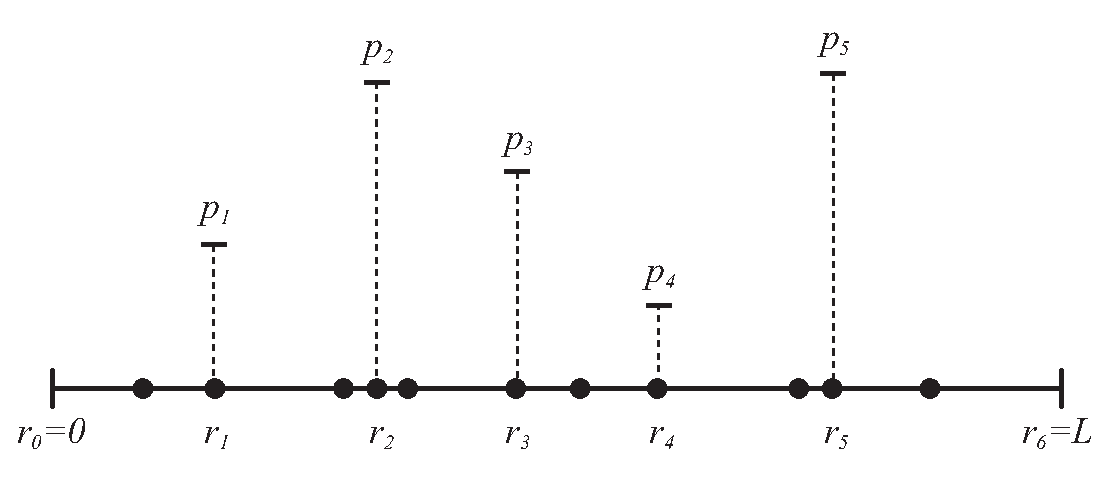
\includegraphics[scale=0.7]{ratesprobs.eps}\hfil
\caption{Plot of the unnormalized relative rates ($r_i$) for each of $\ncat = 5$ categories ($i=1, 2, \cdots, \ncat$). The lower endpoint ($r_0$) always equals 0 and the upper endpoint ($r_{\ncat+1}$) always equals $L$. Neither $r_0$ nor $r_{\ncat+1}$ corresponds to a relative rate, but they are labeled like relative rates in order to facilitate discussion of reversible-jump proposals. The upper bound $L$ is an arbitrary positive real number. The $\ncat$ probabilities associated with the $\ncat$ rates are labeled $p_i$, $i=1,2,\cdots,\ncat$.}
\label{ratesprobs}
\end{figure}

\subsection{Prior on unnormalized probabilities}

The rate probabilities do not require special treatment. These are easily individually updated with a univariate slice sampler \citep{Neal2003a} using a suitably vague prior. These unnormalized probabilities are not used in the likelihood function directly. Instead, a copy of the vector of rate probability parameters is made and the elements of the copy are adjusted to sum to 1.0. The normalized copy now contains valid probabilities that can be used in the likelihood function. Using a Gamma(a, 1.0) prior for each probability parameter is thus equivalent to using a Dirichlet(a, a, $\cdots$, a) prior for the normalized probability vector.

\subsection{Prior on unnormalized rates}

The parameters representing the unnormalized relative rates could be sampled in much the same way, with the normalization ensuring that the relative rates actually used in the likelihood function have mean 1.0. Because reversible jump will be used to change the number of rate categories, however, it is helpful to use a prior on the rate parameters that encourages them to not approach any of the other rate parameters too closely. Identifiability problems could arise if two rates were allowed to have the exact same value (equivalent to reducing the number of categories by 1). Another identfiability issue arises if two rates are allowed to swap places. While this lack of identifiability among the rate parameters may not be an issue (e.g. if the relative rates themselves are considered nuisance parameters), allowing rates to swap places will have a negative effect on mixing, and may cause the chain to spend an inordinate amount of time adjusting rate probabilities in response to rate swaps. Both of these identifiability issues are resolved by ordering the $\ncat$ unnormalized relative rate parameters $r_i$ (i.e. $0.0 = r_0 < r_1 < r_2 < \cdots < r_{\ncat} < r_{\ncat+1} = L$) and using uniform order statistics to determine the prior on each one conditional on all other rates. The upper bound $L$ is a positive real number the value of which, because of the normalization, is arbitrary. For convenience, the lower ($r_0$) and upper ($r_{\ncat+1}$) bounds are labeled in a manner similar to the relative rates, but they are never used as representative relative rates.

To determine the probability density for an order statistics prior, imagine $2 \ncat + 1$ dots placed along an interval from 0 to $L$ (Figure~\ref{ratesprobs}). The location of each dot is determined by a draw from a Uniform(0,$L$) distribution. The position of every $(s+1)$th dot represents the value of one of the unnormalized relative rate parameters ($s$ is the number of ``spacer'' dots between each adjacent relative rate). The prior probability density for the entire vector of $\ncat$ relative rates illustrated in Figure~\ref{ratesprobs} is proportional to a Dirichlet distribution with $\ncat+1$ parameters (see below for derivation):

\[ L^{-(2\ncat+1)} \; \mbox{Dir}(s+1, s+1, s+1, s+1, s+1, s+1) \]

Conditioning on the number of categories, all of the relative rate parameters can be easily updated using a univariate slice sampler with the above prior. Because all relative rates are fixed except the one being updated, the prior for rate parameter $r_i$ is proportional to:

\[ (r_i - r_{i-1})^s (r_{i+1} - r_i)^s \]

\subsubsection{Order statistics}

The purpose of this section is to derive the joint density of two order statistics. The generalization to the density of more than two order statistics is straightforward. Imagine $n$ values are independently sampled from a Uniform(0,$L$) distribution. Below is an example sample in which $n=6$ and $L=10$:

\begin{center}
\begin{tabular}{ccccccccccc}
$X_1 = 8.6$ & & $X_2 = 4.3$ & & $X_3 = 9.2$ & & $X_4 = 1.7$ & & $X_5 = 2.0$ & & $X_6 = 3.0$
\end{tabular} 
\end{center}

If these values are ordered from lowest to highest, the values become the order statistics $X^{(i)}$:
          
\begin{center}
\begin{tabular}{ccccccccccc}
$X^{(1)} = 1.7$ & & $X^{(2)} = 2.0$ & & $X^{(3)} = 3.0$ & & $X^{(4)} = 4.3$ & & $X^{(5)} = 8.6$ & & $X^{(6)} = 9.2$
\end{tabular} 
\end{center}

Suppose we are interested in the joint density of two of these order statistics, namely $X^{(k)}$ and $X^{(m)}$. For example, what is the probability that $X^{(k)}$ is within the interval $(x, x+dx)$ and $X^{(m)} $ is in the interval $(y, y+dy)$? This translates the multinomial probability that exactly $k-1$ of the $X$s fall in the interval $(0,x)$ AND one $X$ falls in the interval $(x,x+dx)$ AND exactly $m-k-1$ of the $X$s fall in the interval $(x,y)$ AND one $X$ falls in the interval $(y,y+dy)$.

\begin{eqnarray*}
& &P(X^{(k)} \in dx, X^{(m)} \in dy) \\
& & = P(\mbox{$k-1$ in $(0,x)$, one in $dx$, $m-k-1$ in $(x,y)$, one $dy$}) \\
& & = \frac{n!}{(k-1)! \; 1! \; (m-k-1)! \; 1! \; (n-m)!} \\
& & \rule{.2in}{0.in} \cdot
      \left[ F(x) \right]^{k-1}
      \left[ f(x) dx \right]^{1}
      \left[ F(y) - F(x) \right]^{m-k-1}
      \left[ f(y) dy \right]^{1}
      \left[ 1 - F(x) \right]^{n-m}
\end{eqnarray*}

Dividing the above probability by $dx \; dy$ produces the density, which can be written as follows:

\begin{eqnarray*}
f_{X^{(k)}, X^{(m)}}(x,y) & = & f(x) f(y) \frac{F(x)^{k-1} \; \left[ F(y) - F(x) \right]^{m-k-1} \; \left[ 1 - F(y) \right]^{(n+1)-m-1}}{\frac{\Gamma(k) \; \Gamma(m-k) \; \Gamma((n+1)-m)}{\Gamma(n+1)}}
\end{eqnarray*}

If the distribution from which the $X$s were drawn is Uniform(0,L), then the density of each $X$ is $f(x) = 1/L$ and the distribution function is $F(x) = x/L$. Substituting these into the above equation yields:

\begin{eqnarray*}
f_{X^{(k)}, X^{(m)}}(x,y) & = & \left( \frac{1}{L} \right)^2 \frac{\left[ \frac{x}{L} \right]^{k-1} \; \left[ \frac{y-x}{L} \right]^{m-k-1} \; \left[ \frac{L-y}{L} \right]^{(n+1)-m-1}}{\frac{\Gamma(k) \; \Gamma(m-k) \; \Gamma((n+1)-m)}{\Gamma(n+1)}} \\
& = & \left( \frac{1}{L} \right)^n \frac{\left[x\right]^{k-1} \; \left[y-x\right]^{m-k-1} \; \left[L-y\right]^{(n+1)-m-1}}{\frac{\Gamma(k) \; \Gamma(m-k) \; \Gamma((n+1)-m)}{\Gamma(n+1)}}
\end{eqnarray*}

If $L=1$, the above density is Dirichlet($k$, $m-k$, $n-m+1$).

\subsection{Reversible jump proposals}

Changing the number of categories changes the model dimension. For example, changing $\ncat$ from 4 to 3 reduces the number of relative rates by 1 and the number of rate probabilities by 1, yielding a model with 2 fewer parameters than the model having $\ncat = 4$. Such manipulations of model dimension require the development of a reversible jump MCMC proposal \citep{Green1995}. I describe below two such proposals: one increases the number of relative rate categories by 1 (the ADDCAT proposal) and the other, complementary proposal reduces the number of rate categories by 1 (the DELCAT proposal). Given the fact that a decision has been made to propose a change to $\ncat$, the probability of the ADDCAT proposal is $\phi$ and the probability of the LESSCATS proposal is thus $1-\phi$. 

The prior on the number of categories ($\ncat$) is assumed to be Poisson($\lambda$) conditional on $\ncat > 0$:

\[ p(\ncat) = \frac{e^{-\lambda} \; \lambda^{\ncat}}{\left( 1 - e^{-\lambda} \right) {\ncat}!}  \].

% unconditional
% p(x) = lambda^x exp{-lambda} / x!
% p(0) = lambda^0 exp(-lambda) / 0! = exp(-lambda)
% p(1) = lambda^1 exp(-lambda) / 1!
% p(2) = lambda^2 exp(-lambda) / 2!
% p(3) = lambda^3 exp(-lambda) / 3!
% p(4) = lambda^4 exp(-lambda) / 4!
% p(5) = lambda^5 exp(-lambda) / 5!
%
% conditional on x > 0
%                                exp{-lambda}   lambda^x
% p(x|x > 0) = p(x)/p(x > 0) = ---------------- --------
%                              1 - exp(-lambda)    x!
% example for lambda = 1.0:
% p(1) = 0.58  cum = 0.58
% p(2) = 0.29  cum = 0.87
% p(3) = 0.10  cum = 0.97
% p(4) = 0.02  cum = 0.99

% ***********************************************************
% ***********************************************************
% ***********************************************************
% **********************   ADDCAT  **************************
% ***********************************************************
% ***********************************************************
% ***********************************************************

\subsubsection{The ADDCAT proposal}

The ADDCAT proposal will be discussed in the context of Figure~\ref{addcat}, which illustrates a ADDCAT proposal resulting in an increase in the number of rate categories from $\ncat = 2$ to $\ncat' = 3$. The ADDCAT proposal adds one relative rate ($r'_i$) and one rate probability ($p'_i$). The new relative rate is chosen by drawing a Uniform(0, $L$) random deviate $u_1$. That is, $r'_i = u_1 L$. The new value $r'_i$ is guaranteed to be between the two values, $r'_{i-1} \ge r'_0$ and $r'_{i+1} \le r'_{\ncat'+1}$. In this example, the particular value chosen for $u_1$ places the new rate between $r_1$ and $r_2$, therefore $i=2$.

%
% Figure "addcat"
%
%\clearpage
\begin{figure}
\centering
\hfil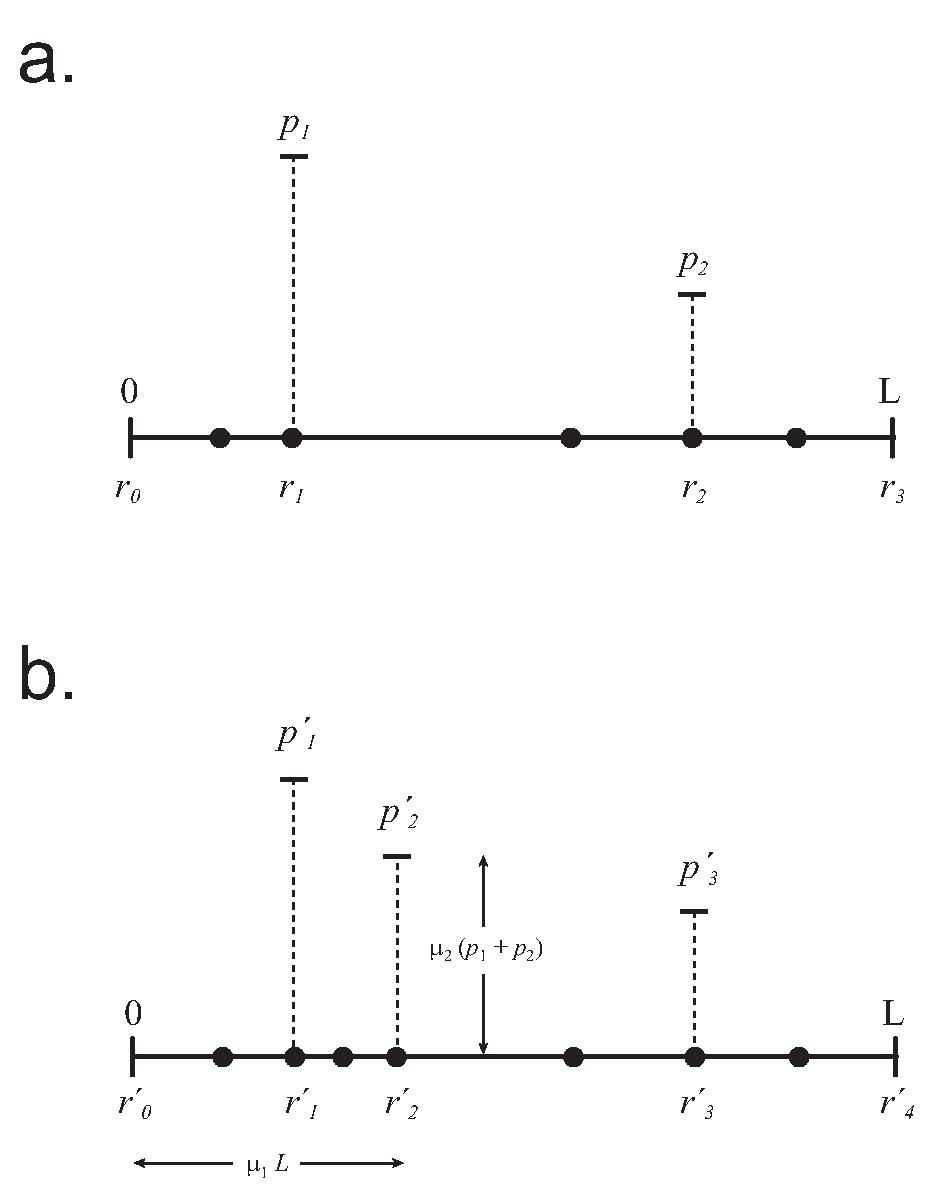
\includegraphics[scale=0.7]{addcat.eps}\hfil
\caption{The ADDCAT proposal changing the number of categories from $\ncat = 2$ to $\ncat = 3$. (a) The 2-category situation before a ADDCAT proposal. (b) The 3-category situation after a ADDCAT proposal in which a new rate ($r'_2$) has been inserted between $r_1$ and $r_2$, which have been renumbered as $r'_1$ and $r'_3$ to accommodate the insertion. A new probability, $p'_2$, has been generated. One Uniform(0,1) random deviate ($u_1$) is used to determine the position of the new rate (i.e. $r'_2 = u_1 L$) and a second Uniform(0,1) random deviate is used to determine the value of $p'_2$(i.e. $p'_2 = u_2*(p_1 + p_2)$).}
\label{addcat}
\end{figure}

The acceptance ratio of a ADDCAT proposal can be described as follows:

\[ R_{\mbox{\tiny ADDCAT}} = \min \left\{1, (\mbox{likelihood ratio}) \times (\mbox{prior ratio}) \times (\mbox{Hastings ratio}) \times (\mbox{Jacobian}) \right\} \]

{\em Likelihood ratio} --- This is the likelihood after the proposal divided by the likelihood before the proposal,

\[ \frac{f(\mbox{data} | {\bf \theta}, {\bf r}', {\bf p}', \ncat')}{f(\mbox{data} | {\bf \theta}, {\bf r}, {\bf p}, \ncat)}. \]

Here, $\theta$ represents all parameters not associated with rate heterogeneity, $\bf r$ and $\bf p$ are the relative rate and rate category probability parameter vectors, respectively, and $\ncat$ is the number of rate categories. A prime symbolizes values of parameters {\em after} the proposal.

{\em Prior ratio} --- The prior ratio is 3-parted:

\[ \mbox{prior ratio} = (\mbox{$\ncat$ prior ratio}) \times (\mbox{rates prior ratio}) \times (\mbox{probs. prior ratio}) \]

The $\ncat$ prior ratio equals the prior probability of $\ncat'$ rate categories divided by the prior probability of $\ncat$ categories:

\begin{eqnarray*}
\mbox{$\ncat$ prior ratio} & = & \frac{\frac{e^{-\lambda} \; \lambda^{\ncat'}}{\left( 1 - e^{-\lambda} \right) {\ncat'}!}}{\frac{e^{-\lambda} \; \lambda^{\ncat}}{\left( 1 - e^{-\lambda} \right) {\ncat}!}} =  \frac{\lambda}{\ncat'}
\end{eqnarray*}

The rates prior ratio equals the joint prior probability density of all $\ncat'$ rate parameters after the proposal divided by the joint prior of the $\ncat$ rate parameters before the proposal. If the new rate $r'_i$ is inserted between the previous rates $r_{i-1}$ and $r_i$,
\begin{eqnarray*}
\mbox{rates prior ratio} 
  & = & \frac
  {
    \left( \frac{1}{L} \right)^{(s+1) \ncat' + 1} \; 
    \frac{ \Gamma\left( (s+1) (\ncat' + 1) \right) }{ \left[ \Gamma(s+1) \right]^{\ncat' + 1} } \;
    \prod_{k=1}^{\ncat' + 1} ({r'}_k - {r'}_{k-1})^s
  }
  {
    \left( \frac{1}{L} \right)^{(s+1) \ncat + 1}
    \frac{ \Gamma\left( (s+1) (\ncat + 1) \right) }{ \left[ \Gamma(s+1) \right]^{\ncat + 1} } \;
    \prod_{k=1}^{\ncat + 1} (r_k - r_{k-1})^s
  } \\
  & = & \left[ L^{s+1} \; \Gamma(s+1)\right]^{-1} \; 
  \left[ \frac{\Gamma\left( (s+1) (\ncat + 2) \right)}{\Gamma\left( (s+1) (\ncat + 1) \right)} \right] \;
  \left[ \frac{(r'_i - r'_{i-1})^s \; (r'_{i+1} - r'_i)^s}{(r_i - r_{i-1})^s} \right]
\end{eqnarray*}

Note that $r_{i-1}$ is not actually a rate parameter if $i=1$, and $r_i$ is not actually a rate parameter if $i=\ncat+1$. If the number of spacers between each $r_i$ is $s=1$, the rates prior ratio simplifies to:
\begin{eqnarray*}
\mbox{rates prior ratio} & = & \frac{(2 \ncat + 4)(2 \ncat + 3)}{L^2} \; 
  \left[ \frac{(r'_i - r'_{i-1}) \; (r'_{i+1} - r'_i)}{(r_i - r_{i-1})} \right]
\end{eqnarray*}

The probabilities prior ratio equals the joint prior probability density of all $\ncat'$ category probability parameters after the proposal divided by the joint prior of the $\ncat$ probability parameters before the proposal. Each probability parameter is assumed to have a Gamma(a,b) prior. During a ADDCAT proposal, none of the original probability parameters change value: if the new rate $r'_i$ has been inserted between rates $r_{i-1}$ and $r_i$, then $p_{i-1}$ becomes $p'_{i-1}$, $p_i$ becomes $p'_{i+1}$, and a new probability $p'_i$ is created. Thus, the probability parameter prior ``ratio'' is really just the prior density of the new parameter $p'_i$:
%\begin{eqnarray*}
%\mbox{probs. prior ratio} & = & 
%  \frac{ 
%         \left[ \frac{ {p'}_{i-1}^{a-1} \; e^{-p'_{i-1}/b} }{ b^a \; \Gamma(a) } \right] \; 
%         \left[ \frac{ {p'}_i^{a-1}     \; e^{-p'_i/b}     }{ b^a \; \Gamma(a) } \right] \;  
%         \left[ \frac{ {p'}_{i+1}^{a-1} \; e^{-p'_{i+1}/b} }{ b^a \; \Gamma(a) } \right]
%       }
%       {
%         \left[ \frac{ p_{i-1}^{a-1}  \; e^{-p_{i-1}/b}  }{ b^a \; \Gamma(a) } \right] \; 
%         \left[ \frac{ p_i^{a-1}      \; e^{-p_i/b}     }{ b^a \; \Gamma(a) } \right]
%       } \\
%& = & 
%   \frac{ e^{(p_{i-1} + p_i - {p'}_{i-1} - {p'}_i - {p'}_{i+1})/b} } { b^a \; \Gamma(a) } \;
%   \left[ \frac{{p'}_{i-1} \; {p'}_i \; {p'}_{i+1}}{p_{i-1} \; p_i} \right]^{a-1}
%\end{eqnarray*}
%If none of the original probability parameters changes value (simplest case), then the probability prior ratio is simply:
\begin{eqnarray*}
\mbox{probs. prior ratio} & = & \frac{ {p'}_i^{a-1} \; e^{-p'_i/b} }{ b^a \; \Gamma(a) } 
\end{eqnarray*}

{\em Hastings ratio} --- Here are the steps involved with the ADDCAT proposal:
\begin{itemize}
\item Choose to perform a ADDCAT move rather than a DELCAT move (probability $\phi$)
\item Choose a Uniform(0,1) random deviate $u_1$ and determine where the new relative rate will go ($u_1 L$). The existing rate to the left of this point will be called $r_{i-1}$ and the next rate to the right of this point will be $r_i$.
\item Choose a second Uniform(0,1) random deviate $u_2$ to determine the unnormalized probability parameter associated with the new category. The new probability parameter ($p'_i$) will be $u_2*(p_{i-1} + p_i)$. This has the effect of making the new probability parameter possibly smaller or larger than either of the neighboring probability parameters, but never more than twice as large as the largest neighboring probability parameter. This is almost certainly less than optimal, but has the benefit of simplicity. 
\end{itemize}

Thus, the total probability density of the ADDCAT proposal is simply $\phi$ because both $u_1$ and $u_2$ are Uniform(0,1). To compute the Hastings ratio, we also need the probability density of the reverse (DELCAT) proposal. To exactly reverse the ADDCAT proposal, we need to perform the following steps in order to eliminate the rate parameter $r'_i$:

\begin{itemize}
\item Choose to perform a DELCAT move rather than a ADDCAT move (probability $1-\phi$)
\item Choose a specific rate to eliminate. There are $\ncat'$ total rate parameters, so the probability we will randomly choose to eliminate $r'_i$ is $1/\ncat'$.
\end{itemize}

The Hastings ratio is thus:

\[ \mbox{Hastings ratio} = \frac{(1-\phi)(1/\ncat')}{\phi} \]

{\em Jacobian} --- To determine the Jacobian, first enumerate all parameters that exist before and after the ADDCAT proposal. We can leave out parameters that have the same numerical value before and after. For example, $r_{i}$ is the same parameter as $r'_{i+1}$, only the labeling is different. The random deviates used to ``invent'' the parameters created during the ADDCAT proposal take the place of those parameters in the ``before'' category.

\begin{center}
\begin{tabular}{lcc}
Before & $u_1$  & $u_2$ \\
After  & $r'_i$ & $p'_i$
\end{tabular}
\end{center}

The Jacobian (absolute value of the determinant of the matrix of derivatives of the ``after'' parameters with respect to the ``before'' parameters) is thus

\begin{eqnarray*}
J = \left| 
\begin{array}{ccc}
\frac{d r'_i}{d u_1} & & \frac{d p'_i}{d u_1} \\
& & \\
\frac{d r'_i}{d u_2} & & \frac{d p'_i}{d u_2}
\end{array}
\right|
= \left| \frac{d r'_i}{d u_1} \; \frac{d p'_i}{d u_2} - \frac{d r'_i}{d u_2} \; \frac{d p'_i}{d u_1} \right|
\end{eqnarray*}

The derivative of $r'_i$ with respect to $u_1$ is

\begin{eqnarray*}
\frac{d r'_i}{d u_1} & = & \frac{d (u_1 L)}{d u_1} \\
& = & L
\end{eqnarray*}

The derivative of $p'_i$ with respect to $u_2$ is

\begin{eqnarray*}
\frac{d p'_i}{d u_2} & = & \frac{d (u_2*(p_{i-1} + p_i))}{d u_2} \\
& = & p_{i-1} + p_i
\end{eqnarray*}

The derivative of $r'_i$ with respect to $u_2$ is 

\begin{eqnarray*}
\frac{d r'_i}{d u_2} & = & 0
\end{eqnarray*}

The derivative of $p'_i$ with respect to $u_1$ is

\begin{eqnarray*}
\frac{d p'_i}{d u_1} & = & 0
\end{eqnarray*}

Putting these together yields

\begin{eqnarray*}
J & = & \left| \frac{d r'_i}{d u_1} \; \frac{d p'_i}{d u_2} - \frac{d r'_i}{d u_2} \; \frac{d p'_i}{d u_1} \right| \\
& = & \left| (L)(p_{i-1} + p_i) - (0)(0) \right| \\
& = & L(p_{i-1} + p_i)
\end{eqnarray*}

{\em Acceptance ratio} --- Multiplying the likelihood ratio, prior ratio, Hastings ratio and Jacobian together yields:

\begin{eqnarray*}
% likelihood ratio
& & \left\{ 
  \frac{f(\mbox{data} | {\bf \theta}, {\bf r}', {\bf p}', \ncat')}{f(\mbox{data} | {\bf \theta}, {\bf r}, {\bf p}, \ncat)} 
\right\}
% ncat prior ratio
\left\{ 
  \frac{\lambda}{\ncat'} 
\right\} \\
& & \rule{.2in}{.0in} \cdot 
% rates prior ratio
\left\{ 
  \left[ L^{s+1} \; \Gamma(s+1)\right]^{-1} \; 
    \left[ \frac{\Gamma\left( (s+1) (\ncat + 2) \right)}{\Gamma\left( (s+1) (\ncat + 1) \right)} \right] \;
    \left[ \frac{(r'_i - r'_{i-1})^s \; (r'_{i+1} - r'_i)^s}{(r_i - r_{i-1})^s} \right]
\right\} \\
& & \rule{.2in}{.0in} \cdot 
% probs prior ratio
\left\{ 
  \frac{ {p'}_i^{a-1} \; e^{-p'_i/b} }{ b^a \; \Gamma(a) } 
\right\} 
% Hastings ratio
\left\{ 
  \frac{(1-\phi)(1/\ncat')}{\phi} 
\right\}
% Jacobian
\left\{ 
  L(p_{i-1} + p_i) 
\right\}
\end{eqnarray*}

% ***********************************************************
% ***********************************************************
% ***********************************************************
% **********************   DELCAT  **************************
% ***********************************************************
% ***********************************************************
% ***********************************************************

\subsubsection{The DELCAT proposal}

This is largely the inverse of the ADDCAT proposal, so most of the derivation and explanation has already been done in the previous section. Figure~\ref{delcat} illustrates a case in which 3 categories is reduced to 2 categories by a DELCAT proposal in which rate $r_i$ is eliminated along with its associated probability $p_i$.

%
% Figure "delcat"
%
%\clearpage
\begin{figure}
\centering
\hfil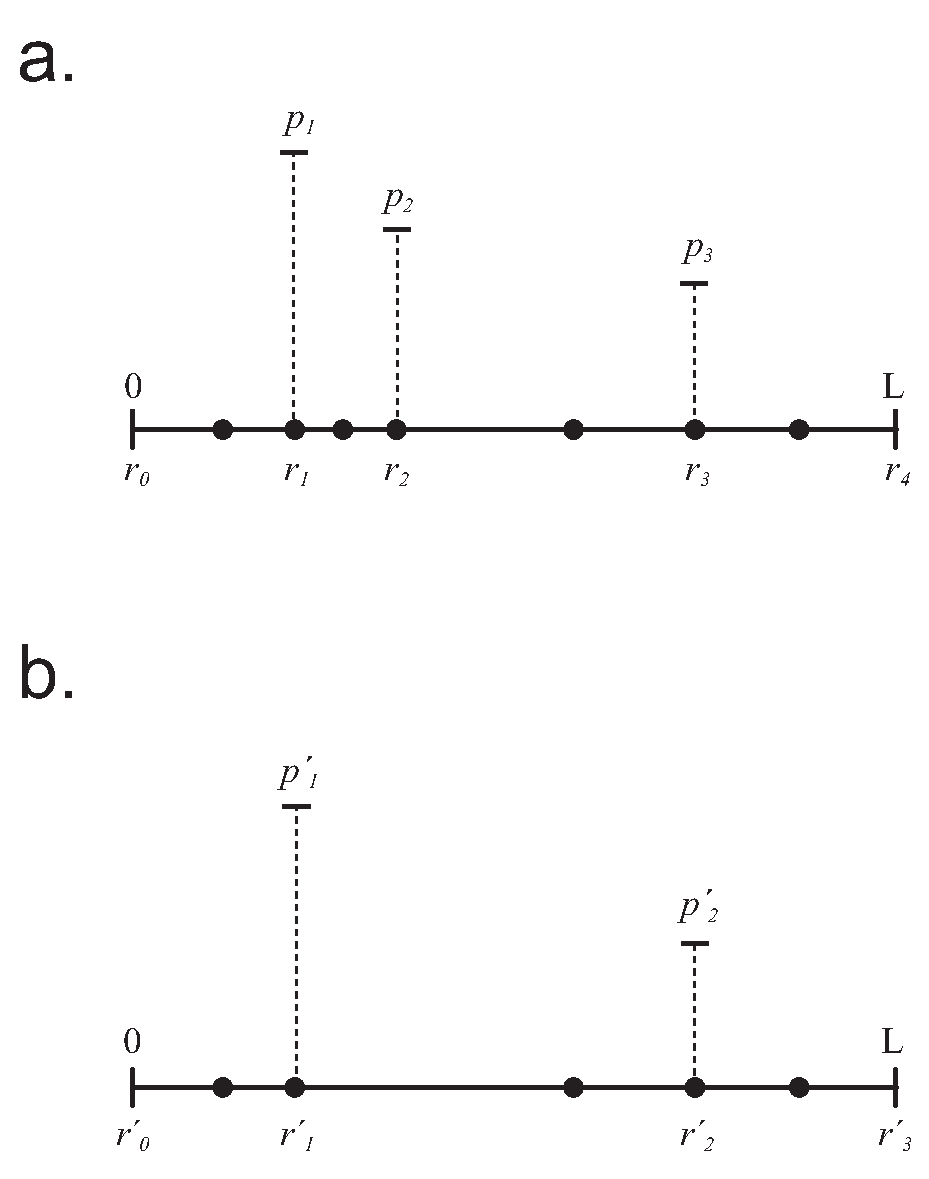
\includegraphics[scale=0.7]{delcat.eps}\hfil
\caption{The DELCAT proposal changing the number of categories from $\ncat = 3$ to $\ncat = 2$. (a) The 3-category situation before a DELCAT proposal. (b) The 2-category situation after a DELCAT proposal in which one of the original rates ($r_2$) and category probabilities ($p_2$) have been deleted.}
\label{delcat}
\end{figure}

The acceptance ratio of a DELCAT proposal can be described as follows:

\[ R_{\mbox{\tiny DELCAT}} = \min \left\{1, (\mbox{likelihood ratio}) \times (\mbox{prior ratio}) \times (\mbox{Hastings ratio}) \times (\mbox{Jacobian}) \right\} \]

\[ \mbox{Likelihood ratio} = \frac{f(\mbox{data} | {\bf \theta}, {\bf r}', {\bf p}', \ncat')}{f(\mbox{data} | {\bf \theta}, {\bf r}, {\bf p}, \ncat)}. \]

\begin{eqnarray*}
\mbox{$\ncat$ prior ratio} & = & \frac{\frac{e^{-\lambda} \; \lambda^{\ncat'}}{\left( 1 - e^{-\lambda} \right) {\ncat'}!}}{\frac{e^{-\lambda} \; \lambda^{\ncat}}{\left( 1 - e^{-\lambda} \right) {\ncat}!}} = \frac{\ncat}{\lambda}
\end{eqnarray*}

\begin{eqnarray*}
\mbox{Rates prior ratio} 
  & = & \left[ L^{s+1} \; \Gamma(s+1)\right] \; 
  \left[ \frac{\Gamma\left( (s+1) (\ncat) \right)}{\Gamma\left( (s+1) (\ncat + 1) \right)} \right] \;
  \left[ \frac{(r'_i - r'_{i-1})^s}{(r_i - r_{i-1})^s \; (r_{i+1} - r_i)^s} \right]
\end{eqnarray*}

\begin{eqnarray*}
\mbox{Probs. prior ratio} & = & \frac{ b^a \; \Gamma(a) }{ {p'}_i^{a-1} \; e^{-p'_i/b} } 
\end{eqnarray*}

\[ \mbox{Hastings ratio} = \frac{\phi}{(1-\phi)(1/\ncat)} \]

\begin{eqnarray*}
\mbox{Jacobian} & = & \left| \frac{d u'_1}{d r_2} \; \frac{d u'_2}{d p_2} - \frac{d u'_2}{d r_2} \; \frac{d u'_1}{d p_2} \right| \\
& = & \left| \left( \frac{1}{L} \right) \left( \frac{1}{p'_{i-1} + p'_i} \right) - (0)(0) \right| \\
& = & \frac{1}{L(p'_{i-1} + p'_i)}
\end{eqnarray*}

{\em Acceptance ratio} --- Multiplying the likelihood ratio, prior ratio, Hastings ratio and Jacobian together yields:

\begin{eqnarray*}
% likelihood ratio
& & \left\{ 
  \frac{f(\mbox{data} | {\bf \theta}, {\bf r}', {\bf p}', \ncat')}{f(\mbox{data} | {\bf \theta}, {\bf r}, {\bf p}, \ncat)} 
\right\}
% ncat prior ratio
\left\{ 
  \frac{\ncat}{\lambda} 
\right\} \\
& & \rule{.2in}{.0in} \cdot 
% rates prior ratio
\left\{ 
  \left[ L^{s+1} \; \Gamma(s+1)\right] \; 
  \left[ \frac{\Gamma\left( (s+1) (\ncat) \right)}{\Gamma\left( (s+1) (\ncat + 1) \right)} \right] \;
  \left[ \frac{(r'_i - r'_{i-1})^s}{(r_i - r_{i-1})^s \; (r_{i+1} - r_i)^s} \right]
\right\} \\
& & \rule{.2in}{.0in} \cdot 
% probs prior ratio
\left\{ 
  \frac{ b^a \; \Gamma(a) }{ {p'}_i^{a-1} \; e^{-p'_i/b} } 
\right\} 
% Hastings ratio
\left\{ 
  \frac{\phi}{(1-\phi)(1/\ncat)} 
\right\}
% Jacobian
\left\{ 
  \frac{1}{L(p'_{i-1} + p'_i)} 
\right\}
\end{eqnarray*}

\section{References}
\renewcommand{\bibsection}{}
\bibliography{flexcat}

\end{document}
